\subsection{Strategic Advantage Condition in Classification}

We now sharpen our problem formulation (Section~\ref{sec:problem_formulation}) for the classification setup and only mention the difference.

The outcome space $\cY = \{-1,+1\}$ is the space of discrete labels and the loss function $\ell(y, \hat{y}) = \Ind{\hat{y} \neq y}$ is the $0$-$1$ loss. In the mandatory disclosure setup, the Sender always chooses $A=X$. For a Receiver strategy defined by $\hat{y}_V(\emptyset) = \sgn(\E[Y])$ and $\hat{y}_V(x) = \sgn(\E[Y|X=x])$, we characterize the vanilla resulting risk in the following lemma.

\begin{lemma}[Classification Vanilla Risk] \label{lem:rv_classification}
In the mandatory disclosure setup, the expected vanilla risk with noisy channel $q$ is
\begin{align}
R_V^\star(q) &= q\Prob(Y=-\sgn(\E[Y])) \nonumber \\
& + (1-q)\E\Big[\frac{1-|\eta(X)|}{2}\Big], \label{eq:rv_classification}
\end{align}
where $\eta(X) = \E[Y|X=x]$.
\end{lemma}

In the voluntary disclosure setup, the Receiver commits to a default prediction $\yhatempt = i \in \{-1, +1\}$, which we refer to as the default option. A Sender with preference $u$ observes $(x, u)$ and chooses whether to disclose $x$. Under the $0$-$1$ loss, the Sender withholds the feature if the default option matches their preference ($u = i$) and discloses it if $u = -i$ to potentially shift the prediction. If the Receiver observes the message $M=X$, the disclosure reveals that $u = -i$, prompting the Receiver to use the optimal posterior predictor $\yhatx = \sgn(\E[Y \mid X=x, U=-i])$.

Because the optimum Receiver strategies are governed entirely by their choice of the default option $i$, there are only two possible strategies in the voluntary setup. Let us analyze each of them. Assuming without loss of generality that $\E[Y] > 0$, we denote the strategy where the default option matches the sign of the prior mean as $\cS_1$ (i.e., $i = 1$) and the alternative strategy as $\cS_{-1}$. We characterize the resulting strategic risk for both of these cases in the following lemma.

\begin{lemma}[Strategic Classification Risk] \label{lem:rs_classification}
For a default prediction $i \in \{-1, 1\}$, let $\pi_i = \Prob(U=i)$ and $\eta_{-i}(X) = \E[Y \mid X, U=-i]$. The strategic risk $R_{\cS_i}^\star(q)$ is:
\begin{align}
R_{\cS_i}^\star(q) &= \pi_i \Prob(Y = -i \mid U=i) \nonumber \\
&\quad + \pi_{-i} \biggl[ (1-q) \E \left[ \frac{1-|\eta_{-i}(X)|}{2} \right] \nonumber \\
&\quad + q \Prob(Y = -i \mid U = -i) \biggr]. \label{eq:rs_classification}
\end{align}
\end{lemma}

To determine the Stackelberg equilibrium, the Receiver must select the strategy $\cS_i$ that has the minimum risk, i.e., $R_S^\star(q) = \min_i R_{\cS_i}^\star(q)$. Since the channel noise parameter $q$ acts linearly on the risk functions, we can characterize the optimal policy based on the value of $q$. By substituting the risk expressions from Lemmas~\ref{lem:rv_classification} and~\ref{lem:rs_classification}, we formally characterize both the Stackelberg equilibrium and the conditions for strategic advantage.

\begin{theorem}[Stackelberg Equilibrium and Strategic Advantage] \label{thm:advantage_classification}
Assume $\E[Y] > 0$. At the maximum noise limit ($q=1$), $\cS_1$ is strictly better (i.e., $R_{\cS_1}^\star(1) < R_{\cS_{-1}}^\star(1)$). At $q=0$, the optimal strategy depends on the underlying distributions, leading to two possible scenarios:
\begin{enumerate}
    \item If $R_{\cS_1}^\star(0) \le R_{\cS_{-1}}^\star(0)$, then $\cS_1$ is the Stackelberg strategy for all $q \in [0, 1]$. The strategic advantage condition $R_V^\star(q) > R_S^\star(q)$ simplifies to:
    \begin{align}
        &(1-q) \biggl[ \E\Big[\frac{1-|\eta(X)|}{2}\Big] - \pi_{-1}\E\Big[\frac{1-|\eta_{-1}(X)|}{2}\Big] \nonumber \\
        &- \pi_1 \Prob(Y=-1 \mid U=1) \biggr] > 0. \label{eq:adv_case1}
    \end{align}
    \item If $\cS_{-1}$ is better at $q=0$ (i.e., $R_{\cS_1}^\star(0) > R_{\cS_{-1}}^\star(0)$), there exists an intermediate threshold $q^\star \in [0, 1]$ given by 
    \begin{align}
    q^\star = \frac{R_{\cS_1}^\star(0) - R_{\cS_{-1}}^\star(0)}{(R_{\cS_{-1}}^\star(1) - R_{\cS_{-1}}^\star(0)) - (R_{\cS_1}^\star(1) - R_{\cS_1}^\star(0))},
    \end{align}
    such that for $q \ge q^\star$, $\cS_1$ is the Stackelberg strategy and the advantage condition is identical to \eqref{eq:adv_case1}. For $q < q^\star$, $\cS_{-1}$ is the Stackelberg strategy, and the strategic advantage requires:
    \begin{align}
        &(1-q)\biggl[\E\Big[\frac{1-|\eta(X)|}{2}\Big] - \pi_1\E\Big[\frac{1-|\eta_1(X)|}{2}\Big]\biggr] \nonumber \\
        &+ q\biggl[\Prob(Y=-1) - \pi_1\Prob(Y=1 \mid U=1)\biggr] \nonumber \\
        &> \pi_{-1}\Prob(Y=1 \mid U=-1). \label{eq:adv_case2}
    \end{align}
\end{enumerate}
\end{theorem}

\begin{remark}
In case~(1) of Theorem~\ref{thm:advantage_classification}, the condition in~\eqref{eq:adv_case1} is independent of $q$: the channel noise parameter only scales the magnitude of the advantage via the $(1-q)$ factor, analogous to the regression setting. In contrast, in case~(2), the condition in~\eqref{eq:adv_case2} explicitly depends on $q$, meaning the channel noise governs both the magnitude and the direction of the strategic advantage.
\end{remark}

\begin{figure}[htpb]
  \centering
  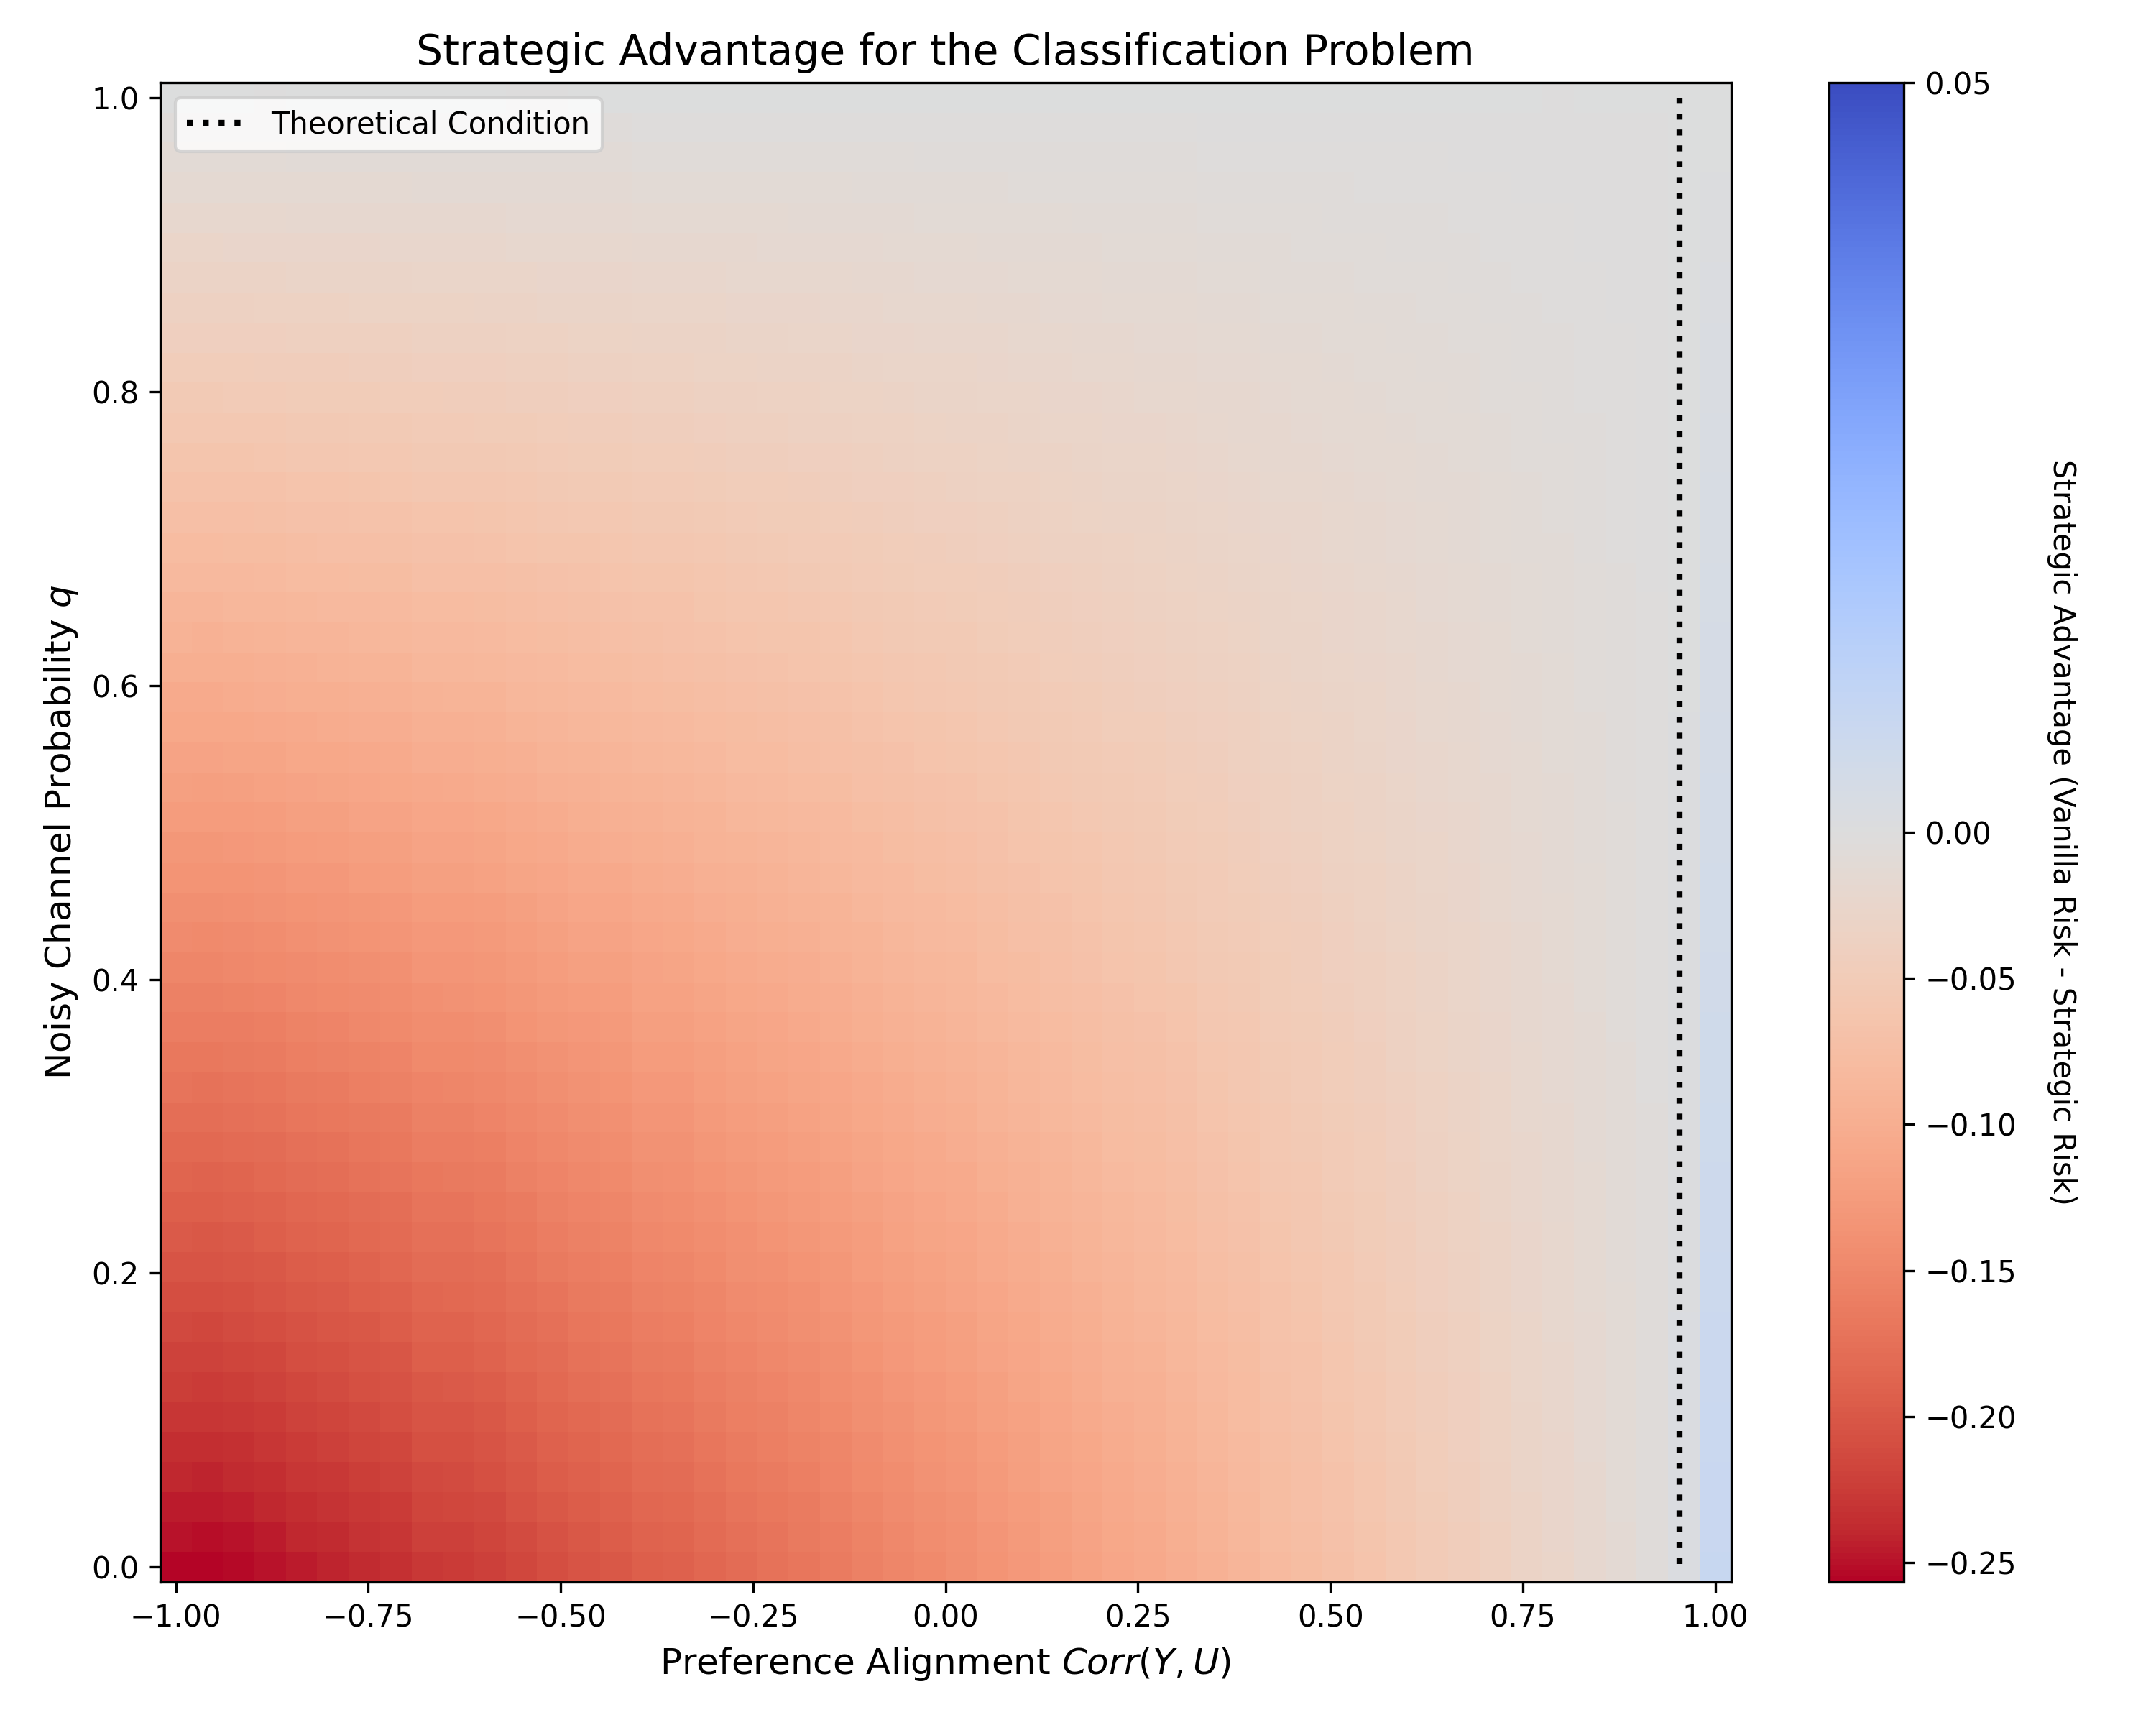
\includegraphics[width=\linewidth]{figures/classification_strategic_advantage.png}
  \caption{Heatmap of the strategic advantage ($R_V^\star(q) - R_S^\star(q) > 0$) for the classification problem. 
  The parameter space sweeps the noisy channel probability $q$ along the y-axis and the discrete preference alignment $\text{Corr}(Y, U)$ along the x-axis. The dotted black contour delineates the theoretical condition boundary from Theorem~\ref{thm:advantage_classification}.}
  \label{fig:classification_conditions}
\end{figure}

To empirically verify these theoretical results, we simulate the classification regime over a family of distributions. We assume discrete labels $(Y,U) \in \{-1, 1\}^2$ sampled from a joint distribution with fixed marginals $P(Y=1) = 0.6$ and $P(U=1) = 0.5$, while we vary $\Cov(Y,U)$ as the varying parameter. The features follow a Gaussian mixture model $X \mid Y, U \sim Y\mu_Y + U\mu_U + \mathcal{N}(0, 1)$, with $\mu_Y = 1.5$ and $\mu_U = 0.5$. To explore the parameter space, we sweep the channel noise probability $q \in [0, 1]$ and the alignment $\Cov(Y,U) \in [-1, 1]$. At each point on the grid, the strategic risk $R_S^\star(q)$ is evaluated by selecting the optimal Receiver strategy. As demonstrated in Fig.~\ref{fig:classification_conditions}, the analytical boundary reliably delineates the regions of strategic advantage.